% SPDX-License-Identifier: CC-BY-SA-4.0
%
% Copyright (c) 2020 Philipp Le
%
% Except where otherwise noted, this work is licensed under a
% Creative Commons Attribution-ShareAlike 4.0 License.
%
% Please find the full copy of the licence at:
% https://creativecommons.org/licenses/by-sa/4.0/legalcode

\phantomsection
\addcontentsline{toc}{section}{Exercise 4}
\section*{Exercise 4}

%%%%%%%%%%%%%%%%%%%%%%%%%%%%%%%%%%%%%%%%%%%%%%%%%%%%%%%%%%%%%%%%%%%%%%%%%%%%%%%
\begin{question}[subtitle={Sampling Periodic Signals}]
	\begin{equation*}
		u(t) = \SI{2}{V} \cdot \cos\left(2\pi \cdot \SI{2}{MHz} \cdot t + \SI{60}{\degree}\right)
	\end{equation*}
	The signal is sampled with a sampling period of $T_S = \SI{125}{\nano\second}$. The first sample taken is $u(t = 0)$.
	
	\begin{tasks}
		\task
		Plot the function from $t = 0$ to $t = \SI{1}{\micro\second}$!
		
		\task
		Calculate the samples $n = 0 \dots 8$!
		
		\task
		What is the DTFT of the signal?
		
		Hints:
		\begin{equation*}
			\begin{split}
				x[n] = e^{-j a n} &= \underline{X}_{2\pi}\left(e^{-j \phi}\right) = 2 \pi \sum\limits_{l = -\infty}^{\infty} \delta \left(\phi + a - 2\pi l\right) \\
				\cos\left(b\right) &= \frac{1}{2} \left(e^{j b} + e^{-j b}\right)
			\end{split}
		\end{equation*}
		
		\task
		Can the DFT directly applied to the signal? If yes, determine the smallest $N$ and give the values of all $\underline{U}[k]$!
		
		\task
		What is the longest possible sampling period? What must be considered at this sampling period?
		
		\task
		Now, the sampling period is changed to $T_S = \SI{0.5}{\micro\second}$. There is no anti-aliasing filter. The reconstruction filter is an ideal low-pass filter with a cut-off frequency of $\SI{2.5}{MHz}$. Give the reconstructed output function in the time domain! Give an explanation in the frequency domain!
	\end{tasks}
\end{question}

\begin{solution}
	\begin{tasks}
		\task
		\begin{figure}[H]
			\centering
			\begin{tikzpicture}
				\begin{axis}[
					height={0.25\textheight},
					width=0.8\linewidth,
					scale only axis,
					xlabel={$t$ in \si{\micro\second}},
					ylabel={$u(t)$},
					%grid style={line width=.6pt, color=lightgray},
					%grid=both,
					grid=none,
					legend pos=outer north east,
					axis y line=middle,
					axis x line=middle,
					every axis x label/.style={
						at={(ticklabel* cs:1.05)},
						anchor=north,
					},
					every axis y label/.style={
						at={(ticklabel* cs:1.05)},
						anchor=east,
					},
					xmin=-0.1,
					xmax=1.1,
					ymin=-2.2,
					ymax=2.2,
					xtick={0,0.125,...,1},
					%xticklabels={$- \omega_S$, $- \frac{\omega_S}{2}$, $0$, $\frac{\omega_S}{2}$, $\omega_S$},
					%ytick={0},
				]
					\addplot[blue, dashed, smooth, domain=0:1, samples=50] plot(\x, {2*cos(deg(2*pi*2*\x)+60)});
					%\addlegendentry{$u(t)$};
					\pgfplotsinvokeforeach{0,0.125,...,1}{
						\addplot[red] coordinates {(#1,0) (#1,{2*cos(deg(2*pi*2*#1)+60)})};
						\addplot[red, only marks, mark=o] coordinates {(#1,{2*cos(deg(2*pi*2*#1)+60)})};
					}
				\end{axis}
			\end{tikzpicture}
		\end{figure}
	
		\task
		\begin{table}[H]
			\centering
			\begin{tabular}{|l|r|r|r|r|r|r|r|r|r|}
				\hline
				$n$ & $0$ & $1$ & $2$ & $3$ & $4$ & $5$ & $6$ & $7$ & $8$
\\
				\hline
				$t$ in \si{\micro\second} & $0.0$ & $0.125$ & $0.25$ & $0.375$ & $0.5$ & $0.625$ & $0.75$ & $0.875$ & $1.0$
\\
				\hline
				\hline
				$u[n]$ in \si{V} & $1.0$ & $-1.73$ & $-1.0$ & $1.73$ & $1.0$ & $-1.73$ & $-1.0$ & $1.73$ & $1.0$ \\
				\hline
			\end{tabular}
		\end{table}
		
		\task
		$t = n T_S$ due to the sampling:
		\begin{equation*}
			\begin{split}
				u[n] &= \SI{2}{V} \cdot \cos\left(2\pi \cdot \SI{2}{MHz} \cdot n T_S + \SI{60}{\degree}\right) \\
				 &= \SI{1}{V} \cdot \left( e^{j \left(2\pi \cdot \SI{2}{MHz} \cdot n T_S + \SI{60}{\degree}\right)} + e^{-j \left(2\pi \cdot \SI{2}{MHz} \cdot n T_S + \SI{60}{\degree}\right)} \right) \\
				 &= \SI{1}{V} \cdot \left( e^{j \SI{60}{\degree}} \cdot e^{j \cdot 2\pi \cdot \SI{2}{MHz} \cdot n T_S} + e^{-j \SI{60}{\degree}} \cdot e^{-j \cdot 2\pi \cdot \SI{2}{MHz} \cdot n T_S} \right)
			\end{split}
		\end{equation*}
		
		The DTFT is:
		\begin{equation*}
			\begin{split}
				\underline{U}_{2\pi}\left(e^{-j \phi}\right) &= \SI{2}{V} \cdot \pi \sum\limits_{l = -\infty}^{\infty} \left( e^{j \SI{60}{\degree}} \cdot \delta\left(\phi - \left(2\pi \cdot \SI{2}{MHz} \cdot T_S\right) - 2\pi l\right)\right. \\ &\qquad + \left.e^{-j \SI{60}{\degree}} \cdot \delta\left(\phi + \left(2\pi \cdot \SI{2}{MHz} \cdot T_S\right) - 2\pi l\right) \right)
			\end{split}
		\end{equation*}
		
		\task
		Yes, it is periodic with $T_0=\SI{500}{ns}$. This means:
		\begin{equation*}
			N = \frac{T_0}{T_S} = 4
		\end{equation*}
		
		The DFT over $N=4$ is:
		\begin{equation*}
			\begin{split}
				\underline{X}[k] &= \sum\limits_{n=0}^{N-1} \underline{x}[n] \cdot e^{-j 2\pi \frac{k}{N} n}
			\end{split}
		\end{equation*}
		\begin{equation*}
			\begin{split}
				\phi[k] &= 2 \pi \frac{k}{N} \\
				\omega[k] &= \frac{\phi[k]}{T_S} \\
				f[k] &= \frac{\omega[k]}{2 \pi} \\
			\end{split}
		\end{equation*}
		
		\begin{table}[H]
			\centering
			\begin{tabular}{|l|r|r|r|r|}
				\hline
				$k$ & $0$ & $1$ & $2$ & $3$
\\
				\hline
				$k$ (alternate) & $0$ & $1$ & $-2$ & $-1$ \\
				\hline
				\hline
				$\phi[k]$ & $0$ & $1.57 \approx \pi$ & $3.14 \approx 2 \pi \equiv -2\pi$ & $4.71 \approx 3 \pi \equiv -\pi$ \\
				\hline
				$\omega[k]$ & $\SI{0}{{\micro\second}^{-1}}$ & $\SI{12.57}{{\micro\second}^{-1}}$ & $\SI{25.13}{{\micro\second}^{-1}}$ & $\SI{37.7}{{\micro\second}^{-1}}$ \\
				\hline
				$f[k]$ & $\SI{0}{MHz}$ & $\SI{2}{MHz}$ & $\SI{4}{MHz} \equiv \SI{-4}{MHz}$ & $\SI{6}{MHz} \equiv \SI{-2}{MHz}$ \\
				\hline
				\hline
				$\underline{U}[k]$ & $0$ & $(2+3.46j)$ & $0$ & $(2-3.46j)$ \\
				\hline
				$|\underline{U}[k]|$ & $0.0$ & $4.0$ & $0.0$ & $4.0$ \\
				\hline
				$\arg\left(\underline{U}[k]\right)$ & $\SI{3.14}{rad} \approx \SI{360}{\degree}$ & $\SI{1.05}{rad} \approx \SI{60}{\degree}$ & $\SI{3.14}{rad} \approx \SI{360}{\degree}$ & $\SI{-1.05}{rad} \approx \SI{-60}{\degree}$ \\
				\hline
			\end{tabular}
		\end{table}
	
		\task
		\begin{itemize}
			\item Minimum possible sampling frequency is \SI{4}{MHz}. Anything below, will violate the Shannon-Nyquist theorem and cause aliasing.
			\item The longest possible sampling period is therefore \SI{250}{ns}.
			\item At $T_S = \SI{250}{ns}$, the sampling phase must be considered, too.
			\begin{itemize}
				\item It must be shifted by $\SI{+60}{\degree}$, so that the maxima of $u(t)$ are sampled.
				\item This retains the amplitude of \SI{2}{V}.
				\item A timing error will effectively reduce the amplitude of the sampled signal in relation to the original signal.
				\item At a timing error of $\Delta T_S = \SI{125}{ns}$, all samples will be zero, because the Dirac comb used for sampling is orthogonal to the original signal.
			\end{itemize}
		\end{itemize}
	
		\task
		The sampling period of \SI{500}{ns} violates the Shannon-Nyquist theorem and causes aliasing.
		
		\begin{figure}[H]
			\subfloat[Original signal $\underline{U}\left(j\omega\right)$] {
				\centering
				\begin{tikzpicture}
					\begin{axis}[
						height={0.15\textheight},
						width=0.25\linewidth,
						scale only axis,
						xlabel={$\omega$},
						ylabel={$|\underline{U}\left(j\omega\right)|$},
						%grid style={line width=.6pt, color=lightgray},
						%grid=both,
						grid=none,
						legend pos=north east,
						axis y line=middle,
						axis x line=middle,
						every axis x label/.style={
							at={(ticklabel* cs:1.05)},
							anchor=north,
						},
						every axis y label/.style={
							at={(ticklabel* cs:1.05)},
							anchor=east,
						},
						xmin=-1.5,
						xmax=1.5,
						ymin=0,
						ymax=1.2,
						xtick={-1, -0.5, 0, 0.5, 1},
						xticklabels={$- \omega_S$, $- \frac{\omega_S}{2}$, $0$, $\frac{\omega_S}{2}$, $\omega_S$},
						ytick={0},
						%ytick={0, 1},
						%yticklabels={0, $\SI{}$}
					]
						\draw[-latex, red, very thick] (axis cs:1,0) -- (axis cs:1,0.8); %node[left,align=right,anchor=north,rotate=90,yshift=-5mm]{$\arg\left(\underline{U}\left(j\omega_S\right)\right) = \SI{60}{\degree}$};
						\draw[-latex, green, very thick] (axis cs:-1,0) -- (axis cs:-1,0.8); %node[left,align=right,anchor=north,rotate=90,yshift=-5mm]{$\arg\left(\underline{U}\left(-j\omega_S\right)\right) = \SI{-60}{\degree}$};
					\end{axis}
				\end{tikzpicture}
			}
			\hfill
			\subfloat[Spectrum of the Dirac comb $\frac{2 \pi}{T} \Sha_{\frac{2 \pi}{T}}(\omega)$] {
				\centering
				\begin{tikzpicture}
					\begin{axis}[
						height={0.15\textheight},
						width=0.27\linewidth,
						scale only axis,
						xlabel={$t$},
						ylabel={$|\frac{2 \pi}{T} \Sha_{\frac{2 \pi}{T}}(\omega)|$},
						%grid style={line width=.6pt, color=lightgray},
						%grid=both,
						grid=none,
						legend pos=north east,
						axis y line=middle,
						axis x line=middle,
						every axis x label/.style={
							at={(ticklabel* cs:1.05)},
							anchor=north,
						},
						every axis y label/.style={
							at={(ticklabel* cs:1.05)},
							anchor=east,
						},
						xmin=-2.5,
						xmax=2.5,
						ymin=0,
						ymax=1.2,
						xtick={-2, ..., 2},
						xticklabels={$-2 \omega_S$, $- \omega_S$, $0$, $\omega_S$, $2 \omega_S$},
						ytick={0},
					]
						\pgfplotsinvokeforeach{-3, -2, ..., 3}{
							\draw[-latex, blue, very thick] (axis cs:#1,0) -- (axis cs:#1,1);
						}
					\end{axis}
				\end{tikzpicture}
			}
			\hfill
			\subfloat[Sampled signal $\underline{U}_S\left(j\omega\right)$, showing aliasing] {
				\centering
				\begin{tikzpicture}
					\begin{axis}[
						height={0.15\textheight},
						width=0.27\linewidth,
						scale only axis,
						xlabel={$\omega$},
						ylabel={$|\underline{U}_S\left(j\omega\right)|$},
						%grid style={line width=.6pt, color=lightgray},
						%grid=both,
						grid=none,
						legend pos=north east,
						axis y line=middle,
						axis x line=middle,
						every axis x label/.style={
							at={(ticklabel* cs:1.05)},
							anchor=north,
						},
						every axis y label/.style={
							at={(ticklabel* cs:1.05)},
							anchor=east,
						},
						xmin=-2.5,
						xmax=2.5,
						ymin=0,
						ymax=1.2,
						xtick={-2, -1, -0.5, 0, 0.5, 1, 2},
						xticklabels={$-2 \omega_S$, $- \omega_S$, $- \frac{\omega_S}{2}$, $0$, $\frac{\omega_S}{2}$, $\omega_S$, $2 \omega_S$},
						ytick={0},
					]
						\pgfplotsinvokeforeach{-3, -2, ..., 3}{
							\draw[-latex, blue, dashed, very thick] (axis cs:#1,0) -- (axis cs:#1,1);
							\draw[-latex, green, very thick] (axis cs:{#1-0.01},0) -- (axis cs:{#1-0.01},0.8);
							\draw[-latex, red, very thick] (axis cs:{#1+0.01},0) -- (axis cs:{#1+0.01},0.8);
						}
					\end{axis}
				\end{tikzpicture}
			}
		\end{figure}
	
		\begin{itemize}
			\item The spectral components of $\SI{+2}{MHz}$ (with $e^{j \SI{60}{\degree}}$) and $\SI{-2}{MHz}$ (with $e^{j \SI{-60}{\degree}}$) superimpose at \SI{0}{Hz} (DC).
			\item The resulting component at \SI{0}{Hz} is the addition if two complex numbers (see Part c) ):
			\begin{equation*}
				\underline{U}_S\left(j 0\right) = \SI{2}{V} \cdot \pi \underbrace{\left(e^{j \SI{60}{\degree}} + e^{j \SI{-60}{\degree}}\right)}_{= 1}  \delta(\omega) = \SI{2}{V} \cdot \pi \cdot  \delta(\omega)
			\end{equation*}
			\item Applying the reconstruction filter gives the spectrum of the reconstructed signal:
			\begin{equation*}
				\underline{U}_R\left(j \omega\right) = \SI{2}{V} \cdot \pi \cdot \delta(\omega)
			\end{equation*}
			\item The inverse DTFT is:
			\begin{equation*}
				u_R(t) = \SI{1.0}{V}
			\end{equation*}
			\item The reconstructed signal is a DC signal of \SI{1.0}{V}.
		\end{itemize}
	
		\begin{figure}[H]
			\centering
			\begin{tikzpicture}
				\begin{axis}[
					height={0.15\textheight},
					width=0.8\linewidth,
					scale only axis,
					xlabel={$t$ in \si{\micro\second}},
					ylabel={$u(t)$},
					%grid style={line width=.6pt, color=lightgray},
					%grid=both,
					grid=none,
					legend pos=outer north east,
					axis y line=middle,
					axis x line=middle,
					every axis x label/.style={
						at={(ticklabel* cs:1.05)},
						anchor=north,
					},
					every axis y label/.style={
						at={(ticklabel* cs:1.05)},
						anchor=east,
					},
					xmin=-0.1,
					xmax=1.1,
					ymin=-2.2,
					ymax=2.2,
					xtick={0,0.125,...,1},
					%xticklabels={$- \omega_S$, $- \frac{\omega_S}{2}$, $0$, $\frac{\omega_S}{2}$, $\omega_S$},
					%ytick={0},
				]
					\addplot[blue, dashed, smooth, domain=0:1, samples=50] plot(\x, {2*cos(deg(2*pi*2*\x)+60)});
					\addlegendentry{$u(t)$};
					\addplot[olive] coordinates {(0,1) (0.5,1) (1,1)};
					\addlegendentry{$u_R(t)$};
					\pgfplotsinvokeforeach{0,0.5,1}{
						\addplot[red] coordinates {(#1,0) (#1,{2*cos(deg(2*pi*2*#1)+60)})};
						\addplot[red, only marks, mark=o] coordinates {(#1,{2*cos(deg(2*pi*2*#1)+60)})};
					}
				\end{axis}
			\end{tikzpicture}
		\end{figure}
	\end{tasks}
\end{solution}

%%%%%%%%%%%%%%%%%%%%%%%%%%%%%%%%%%%%%%%%%%%%%%%%%%%%%%%%%%%%%%%%%%%%%%%%%%%%%%%
\begin{question}[subtitle={Sampling Non-Periodic Signals}]
	The signal $x[n]$ is given in the time domain.
	\begin{table}[H]
		\centering
		\begin{tabular}{|l|r|r|r|r|r|r|r|r|}
			\hline
			$n$ & 0 & 1 & 2 & 3 & 4 & 5 & 6 & 7 \\
			\hline
			\hline
			$x[n]$ & 0.25 & 1 & -0.5 & 0.5 & -0.5 & -1 & -0.5 & -0.75 \\
			\hline
		\end{tabular}
	\end{table}
	
	\begin{tasks}
		\task
		The signal is windowed with $N = 4$ starting at $x[n = 0]$. A hamming window with $M = 2$ is applied. Calculate the values of $\underline{x}_W[n]$!
		
		Hamming window:
		\begin{equation*}
			w[n] = \begin{cases}0.54 - 0.46 \cos\left(\frac{2 \pi n}{M}\right), &\quad 0 \leq n \leq M,\\ 0, &\quad \text{otherwise}.\end{cases}
		\end{equation*}
		
		\task
		Calculate the discrete Fourier transform of the windowed signal!
		
		\task
		The signal has been sampled with $T_S = \SI{1}{ms}$. What frequency values do the $k$ represent?
	\end{tasks}
\end{question}

\begin{solution}
	\begin{tasks}
		\task
		At first the signal is truncated. Only the first $4$ samples are considered.
		
		The window function is:
		\begin{equation*}
			w[n] = \begin{cases}0.54 - 0.46 \cos\left(\frac{2 \pi n}{M}\right), &\quad 0 \leq n \leq M,\\ 0, &\quad \text{otherwise}.\end{cases}
		\end{equation*}
		
		The signal is then multiplied with the window:
		\begin{equation*}
			x_w[n] = x[n] \cdot w[n]
		\end{equation*}
		
		\begin{table}[H]
			\centering
			\begin{tabular}{|l|r|r|r|r|}
				\hline
				$n$ & 0 & 1 & 2 & 3 \\
				\hline
				\hline
				$w[n]$ & 0.08 & 1.0 & 0.08 & 0 \\
				\hline
				$x_w[n]$ & 0.02 & 1.0 & -0.04 & 0 \\
				\hline
			\end{tabular}
		\end{table}
		
		\task
		The signal is periodically repeated.
		
		The DFT is calculated over $N = 4$.
		\begin{equation*}
			\underline{X}_w[k] = \mathcal{F}_{\text{DFT}}\left\{\underline{x}[n]\right\} = \sum\limits_{n \in N} \underline{x}[n] \cdot e^{-j 2\pi \frac{k}{N} n}
		\end{equation*}
		
		\begin{table}[H]
			\centering
			\begin{tabular}{|l|r|r|r|r|}
				\hline
				$k$ & 0 & 1 & 2 & 3 \\
				\hline
				$k$ (alternate) & 0 & 1 & -2 & -1 \\
				\hline
				\hline
				$\underline{X}_w[k]$ & $0.98$ & $(0.06-1j)$ & $-1.02$ & $(0.06+1j)$ \\
				\hline
				$|\underline{X}_w[k]|$ & $0.98$ & $1.00$ & $1.02$ & $1.00$ \\
				\hline
				$\arg\left(\underline{X}_w[k]\right)$ & $0$ & $-1.51 \approx -\pi$ & $3.14 \approx 2\pi$ & $1.51 \approx \pi$ \\
				\hline
			\end{tabular}
		\end{table}
	
		\task
		\begin{equation*}
			\begin{split}
				\phi[k] &= 2 \pi \frac{k}{N} \\
				\omega[k] &= \frac{\phi[k]}{T_S} \\
				f[k] &= \frac{\omega[k]}{2 \pi} \\
			\end{split}
		\end{equation*}
		
		\begin{table}[H]
			\centering
			\begin{tabular}{|l|r|r|r|r|}
				\hline
				$k$ & 0 & 1 & 2 & 3 \\
				\hline
				$k$ (alternate) & 0 & 1 & -2 & -1 \\
				\hline
				\hline
				$\phi[k]$ & $0$ & $1.57 \approx \pi$ & $3.14 \approx 2 \pi \equiv -2\pi$ & $4.71 \approx 3 \pi \equiv -\pi$ \\
				\hline
				$\omega[k]$ & $\SI{0}{s^{-1}}$ & $\SI{1570.8}{s^{-1}}$ & $\SI{3141.6}{s^{-1}}$ & $\SI{4712.4}{s^{-1}}$ \\
				\hline
				\hline
				$f[k]$ & $\SI{0}{Hz}$ & $\SI{250}{Hz}$ & $\SI{500}{Hz} \equiv \SI{-500}{Hz}$ & $\SI{750}{Hz} \equiv \SI{-250}{Hz}$ \\
				\hline
			\end{tabular}
		\end{table}
	\end{tasks}
\end{solution}

%%%%%%%%%%%%%%%%%%%%%%%%%%%%%%%%%%%%%%%%%%%%%%%%%%%%%%%%%%%%%%%%%%%%%%%%%%%%%%%
\begin{question}[subtitle={Quantization}]
	The signal of Task 1b) is now quantized. The quantizer has $8$ discrete values. These values are equally distributed between \SI{-2}{V} and \SI{2}{V}. Prior to sampling, the original time-continuous signal passed through an ideal low-pass filter with a cut-off frequency of \SI{4}{MHz}.
	
	\begin{tasks}
		\task
		Define a mapping from the value-continuous samples to the value-discrete samples!
		
		\task
		The value-discrete samples are now pulse-code modulated. How many bits are required?
		
		\task
		What is the resulting data (signal from Task 1b) )?
		
		\task
		Determine the quantization error for each value-discrete sample! How much is the signal-to-quantization-noise ratio?
		
		\task
		3 bits are a very poor resolution. How many bits are appropriate for the quantizer to obtain the best signal-to-noise ratio? Effects of the window filter are neglected. Assume that the signal has passed through a processing chain with a total gain of \SI{24}{dB}, noise figure of \SI{12}{dB} and bandwidth of \SI{4}{MHz} prior to quantization. The input of the quantizer has an impedance of \SI{50}{\ohm}. % 14 bits
	\end{tasks}
\end{question}

\begin{solution}
	\begin{tasks}
		\task
		\begin{itemize}
			\item $\hat{U}_L = \SI{-2}{V}$
			\item $\hat{U}_H = \SI{2}{V}$
			\item $K = 8$
		\end{itemize}
		\begin{equation*}
			\Delta \hat{U} = \frac{\hat{U}_H - \hat{U}_L}{K - 1} = \SI{0.57}{V}
		\end{equation*}
		
		The boundaries for the rounding quantizer are distributed $\pm \frac{1}{2} \Delta \hat{U}$ around each mean.
		\begin{table}[H]
			\begin{tabular}{|r|r|r|r|}
				\hline
				From & To & Maps to & PCM data \\
				\hline
				\hline
				$-\infty$ & $\SI{-1.71}{V}$ & $\SI{-2.0}{V}$ & 0
\\
				$\SI{-1.71}{V}$ & $\SI{-1.14}{V}$ & $\SI{-1.43}{V}$ & 1
\\
				$\SI{-1.14}{V}$ & $\SI{-0.57}{V}$ & $\SI{-0.86}{V}$ & 2
\\
				$\SI{-0.57}{V}$ & $\SI{-0.0}{V}$ & $\SI{-0.29}{V}$ & 3
\\
				$\SI{0.0}{V}$ & $\SI{0.57}{V}$ & $\SI{0.29}{V}$ & 4
\\
				$\SI{0.57}{V}$ & $\SI{1.14}{V}$ & $\SI{0.86}{V}$ & 5
\\
				$\SI{1.14}{V}$ & $\SI{1.71}{V}$ & $\SI{1.43}{V}$ & 6
\\
				$\SI{1.71}{V}$ & $\infty$ & $\SI{2.0}{V}$ & 7 \\
				\hline
			\end{tabular}
		\end{table}
	
		\task
		\begin{equation*}
			B \geq \log_2 \left(K\right) = 3
		\end{equation*}
		Minimum 3 bits.
		
		\task
		\begin{table}[H]
			\centering
			\begin{tabular}{|l|r|r|r|r|r|}
				\hline
				$n$ & $0$ & $1$ & $2$ & $3$ & $4$
\\
				\hline
				\hline
				$u[n]$ in \si{V} & $1.0$ & $-1.73$ & $-1.0$ & $1.73$ & $1.0$ \\
				\hline
				Quantized values in \si{V} & $0.86$ & $-2.0$ & $-0.86$ & $2.0$ & $0.86$ \\
				\hline
				PCM data & $\left(101\right)_2$ & $\left(000\right)_2$ & $\left(010\right)_2$ & $\left(111\right)_2$ & $\left(101\right)_2$ \\
				\hline
				\hline
				$n$ & $5$ & $6$ & $7$ & $8$ &
\\
				\hline
				\hline
				$u[n]$ in \si{V} & $-1.73$ & $-1.0$ & $1.73$ & $1.0$ & \\
				\hline
				Quantized values in \si{V} & $-2.0$ & $-0.86$ & $2.0$ & $0.86$ & \\
				\hline
				PCM data & $\left(000\right)_2$ & $\left(010\right)_2$ & $\left(111\right)_2$ & $\left(101\right)_2$ & \\
				\hline
			\end{tabular}
		\end{table}
	
		\task
		\begin{table}[H]
			\centering
			\begin{tabular}{|l|r|r|r|r|r|}
				\hline
				$n$ & $0$ & $1$ & $2$ & $3$ & $4$
\\
				\hline
				\hline
				$u[n]$ in \si{V} & $1.0$ & $-1.73$ & $-1.0$ & $1.73$ & $1.0$ \\
				\hline
				Quantized values in \si{V} & $0.86$ & $-2.0$ & $-0.86$ & $2.0$ & $0.86$ \\
				\hline
				Quantization error in \si{V} & $0.14$ & $0.27$ & $0.14$ & $0.27$ & $0.14$ \\
				\hline
				\hline
				$n$ & $5$ & $6$ & $7$ & $8$ &
\\
				\hline
				\hline
				$u[n]$ in \si{V} & $-1.73$ & $-1.0$ & $1.73$ & $1.0$ & \\
				\hline
				Quantized values in \si{V} & $-2.0$ & $-0.86$ & $2.0$ & $0.86$ & \\
				\hline
				Quantization error in \si{V} & $0.27$ & $0.14$ & $0.27$ & $0.14$ & \\
				\hline
			\end{tabular}
		\end{table}
	
		The signal-to-quantization-noise ratio for the sine wave is:
		\begin{equation*}
			\mathrm{SQNR} = \SI{1.761}{dB} + B \cdot \SI{6.02}{dB} = \SI{19.82}{dB}
		\end{equation*}
		
		\task
		\begin{itemize}
			\item The RMS value of the signal is $U_{\mathrm{RMS}} = \frac{\SI{2}{V}}{\sqrt{2}} = \SI{1.41}{V}$
			\item The signal power is $P_S = \frac{U_{\mathrm{RMS}}^2}{R} = \SI{39.8}{mW} \equiv L_{P,S} = \SI{16}{dBm}$
			\item The thermal noise floor is $\SI{-174}{dBm/Hz}$
			\item At $\SI{4}{MHz} \equiv \SI{66}{dBHz}$, the thermal noise power is $\SI{-174}{dBm/Hz} + \SI{66}{dBHz} = \SI{-108}{dBm}$
			\item The gain and noise factor is applied to the thermal noise, resulting in a noise power of $L_{P,N} = \SI{-108}{dBm} + \SI{24}{dB} + \SI{12}{dB} = \SI{-70}{dBm}$
			\item \textit{Note that the gain is not applied to the signal power, because it is already known/given at the quantizer input.}
			\item The signal-to-noise ratio is $L_{\mathrm{SNR}} = L_{P,S} - L_{P,N} = \SI{16}{dBm} - \SI{-71}{dBm} = \SI{86}{dB}$
			\item The signal-to-quantization-noise ratio should not be grater than the signal-to-noise ratio, because otherwise the thermal noise would dominate the quantization noise.
			\begin{equation*}
				L_{\mathrm{SQNR}} \stackrel{!}{=} L_{\mathrm{SNR}}
			\end{equation*}
			\item The number of bits must be at least
			\begin{equation*}
				B \geq \frac{L_{\mathrm{SQNR}} - \SI{1.761}{dB}}{\SI{6.02}{dB}} = 14
			\end{equation*}
		\end{itemize}
	\end{tasks}
\end{solution}

\begin{question}[subtitle={Python Programming: Quantization}]
Solve all tasks in Python!

Create a sinusoidal signal with an amplitude of 5.0. The signal is now quantized. Each value is rounded to the next integer.

Plot all signals!

Calculate the quantization error and plot it!
\end{question}

\begin{solution}
\end{solution}

%%%%%%%%%%%%%%%%%%%%%%%%%%%%%%%%%%%%%%%%%%%%%%%%%%%%%%%%%%%%%%%%%%%%%%%%%%%%%%%
%\begin{question}[subtitle={Decibel}]
%	\begin{tasks}
%	\end{tasks}
%\end{question}
%
%\begin{solution}
%	\begin{tasks}
%	\end{tasks}
%\end{solution}
